\documentclass{standalone}
\usepackage[utf8]{inputenc}
\usepackage[dvipsnames,svgnames]{xcolor}
\usepackage{tikz}
\usetikzlibrary[ arrows.meta ]

\begin{document}

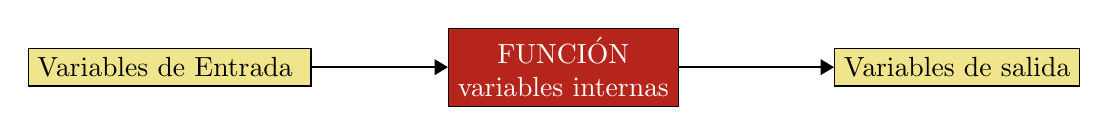
\begin{tikzpicture}[align=center,>=Triangle ]

  %\path [>=latex,draw,black]  (-5,0) node  { Variables de Entrada } 
  %    -> (0,0)  node  {FUNCION} 
  %    -> (5,0) node {Variables de salida} ;
  \node[draw,fill=Khaki] (A) at (-5,0) { Variables de Entrada };
  \node[draw,fill=BrickRed,text=white] (B) at (0,0) 
       {FUNCIÓN \\ variables internas};
  \node[draw,fill=Khaki] (C) at (5,0)  {Variables de salida};
  \draw[-> ,black,thick ] (A) -> (B);
  \draw[->, black,thick] (B) -> (C);


\end{tikzpicture}

\end{document}
